\documentclass[11pt]{article}
\usepackage{geometry,marginnote} % Pour passer au format A4
\geometry{hmargin=1cm, vmargin=1.5cm} % 

% Page et encodage
\usepackage[T1]{fontenc} % Use 8-bit encoding that has 256 glyphs
\usepackage[english,french]{babel} % Français et anglais
\usepackage[utf8]{inputenc} 

\usepackage{lmodern}
\usepackage[np]{numprint}
\setlength\parindent{0pt}

% Graphiques
\usepackage{graphicx,float,grffile}
\usepackage{tikz,pst-eucl,pst-plot,pstricks,pst-node,pstricks-add,pst-fun,pgfplots} 

% Maths et divers
\usepackage{amsmath,amsfonts,amssymb,amsthm,verbatim,scratch3}
\usepackage{multicol,enumitem,url,eurosym,gensymb,tabularx}

\DeclareUnicodeCharacter{20AC}{\euro}



% Sections
\usepackage{sectsty} % Allows customizing section commands
\allsectionsfont{\centering \normalfont\scshape}

% Tête et pied de page
\usepackage{fancyhdr} \pagestyle{fancy} \fancyhead{} \fancyfoot{}

%\fancyfoot[L]{Collège Faubert}
%\fancyfoot[C]{\thepage / 6}
%\fancyfoot[R]{Série Générale}

\renewcommand{\headrulewidth}{0pt} % Remove header underlines
%\renewcommand{\footrulewidth}{0pt} % Remove footer underlines

\newcommand{\horrule}[1]{\rule{\linewidth}{#1}} % Create horizontal rule command with 1 argument of height

\newcommand{\Pointilles}[1][3]{%
  \multido{}{#1}{\makebox[\linewidth]{\dotfill}\\[\parskip]
}}

\newtheorem{Definition}{Définition}

\usepackage{siunitx}
\sisetup{
    detect-all,
    output-decimal-marker={,},
    group-minimum-digits = 3,
    group-separator={~},
    number-unit-separator={~},
    inter-unit-product={~}
}

\setlength{\columnseprule}{1pt}


\begin{document}

\textbf{Nom, Prénom :} \hspace{8cm} \textbf{Classe :} \hspace{3cm} \textbf{Date :}\\

\begin{center}
  \textit{Les propositions mathématiques sont reçues comme vraies parce que personne n’a intérêt qu’elles soient fausses.} - \textbf{Montesquieu}
\end{center}

\textbf{Def : Symétrie axiale : } \dotfill \\ \Pointilles[2] \\

\textbf{Ex 1 : Tracer la symétrie}

\begin{figure}[H]
  \centering
  \includegraphics[width=0.7\linewidth]{6x4-symetrie/ex1b.pdf}
\end{figure}

\begin{multicols}{2} 
\textbf{Ex 2 : Tracer la symétrie}

\begin{figure}[H]
  \centering
  \includegraphics[width=0.4\linewidth]{6x4-symetrie/ex2b.pdf}
\end{figure}

\textbf{Ex 3 : Tracer tous les axes de symétrie}

\begin{figure}[H]
  \centering
  \includegraphics[width=0.9\linewidth]{6x4-symetrie/ex3b.pdf}
\end{figure}
\end{multicols}

\textbf{Ex 4 : Tracer la symétrie}

\begin{multicols}{2} 
\begin{figure}[H]
  \centering
  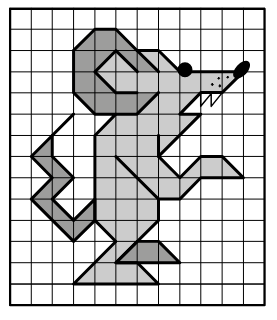
\includegraphics[width=0.6\linewidth]{6x4-symetrie/ex4c.png}
\end{figure}

\begin{figure}[H]
  \centering
  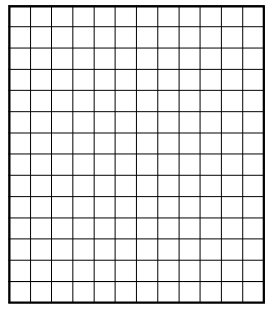
\includegraphics[width=0.6\linewidth]{6x4-symetrie/ex4d.png}
\end{figure}
\end{multicols}

\newpage
\textbf{Ex 5 : Tracer la figure au compas}

\begin{figure}[H]
  \centering
  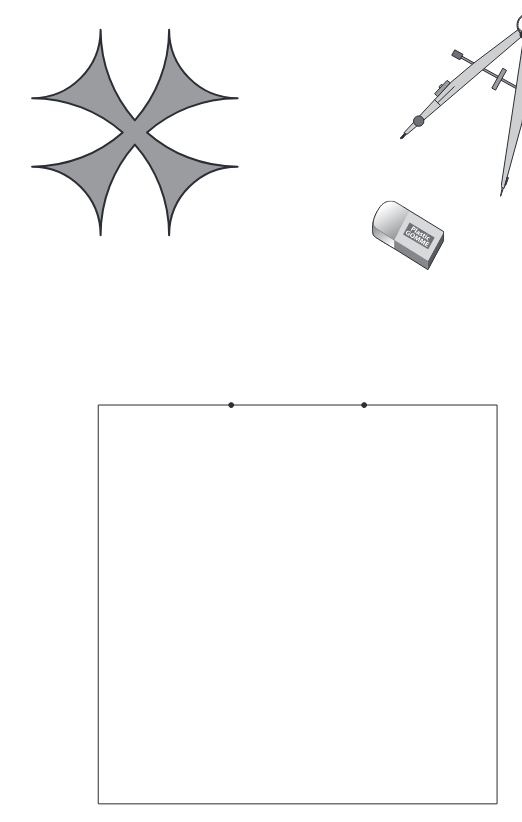
\includegraphics[width=0.8\linewidth]{6x4-symetrie/ex5b.png}
\end{figure}

\newpage

\textbf{Nom, Prénom :} \hspace{8cm} \textbf{Classe :} \hspace{3cm} \textbf{Date :}\\

\begin{center}
  \textit{Les propositions mathématiques sont reçues comme vraies parce que personne n’a intérêt qu’elles soient fausses.} - \textbf{Montesquieu}
\end{center}

\textbf{Def : Symétrie axiale : } \dotfill \\ \Pointilles[2] \\

\textbf{Ex 1 : Tracer la symétrie}

\begin{figure}[H]
  \centering
  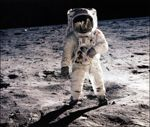
\includegraphics[width=0.7\linewidth]{6x4-symetrie/ex1.pdf}
\end{figure}

\begin{multicols}{2} 
\textbf{Ex 2 : Tracer la symétrie}

\begin{figure}[H]
  \centering
  
\includegraphics[width=0.4\linewidth]{6x4-symetrie/ex2.pdf}
\end{figure}

\textbf{Ex 3 : Tracer tous les axes de symétrie}

\begin{figure}[H]
  \centering
  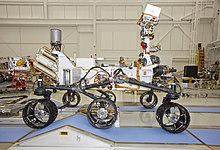
\includegraphics[width=0.9\linewidth]{6x4-symetrie/ex3.pdf}
\end{figure}
\end{multicols}

\textbf{Ex 4 : Tracer la symétrie}

\begin{multicols}{2} 
\begin{figure}[H]
  \centering
  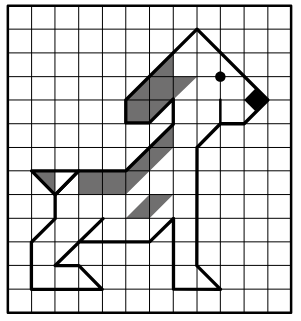
\includegraphics[width=0.6\linewidth]{6x4-symetrie/ex4a.png}
\end{figure}

\begin{figure}[H]
  \centering
  
\includegraphics[width=0.6\linewidth]{6x4-symetrie/ex4b.png}
\end{figure}
\end{multicols}

\newpage
\textbf{Ex 5 : Tracer la figure au compas}

\begin{figure}[H]
  \centering
  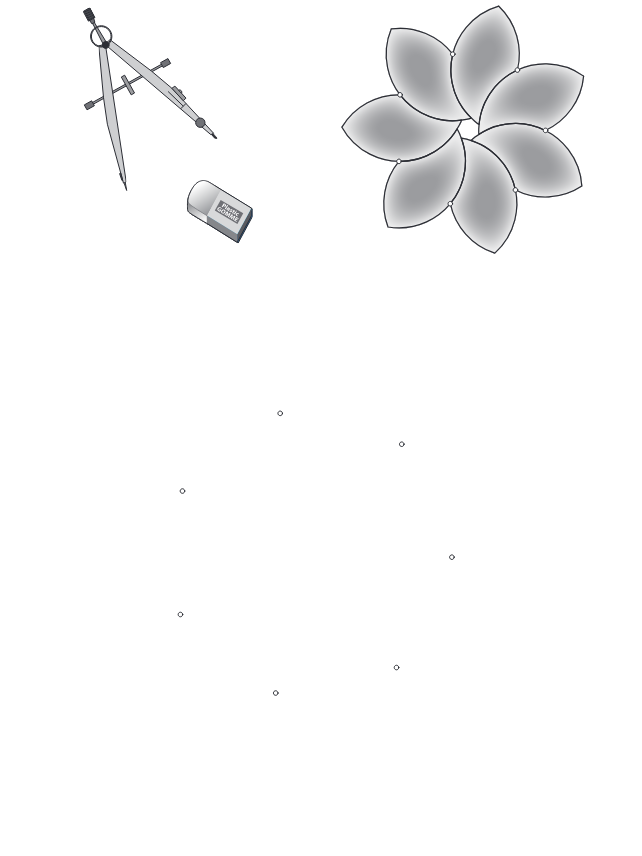
\includegraphics[width=0.9\linewidth]{6x4-symetrie/ex5.png}
\end{figure}

\end{document}